%=============================================================================
% SECTION 9: ATOMIC CLOCK PHENOMENOLOGY
% Part VI: Laboratory Tests
% Equations: (48)-(53)
% Estimated pages: 8-10
%=============================================================================

\section{Atomic Clock Tests}\label{sec:clocks}

Atomic clocks remain one of the sharpest laboratory probes of \DFD.  The key lesson from the recent clock-sector corrections is that one must distinguish \emph{channels}.  Same-ion optical comparisons test the pure electromagnetic-sector coupling; cross-species atomic ratios primarily test composition-sensitive structure; and nuclear clocks uniquely access the strong sector.  General relativity predicts exact universality for co-located clocks after the common redshift is removed.  \DFD instead predicts that the residual differential response is channel-dependent and environment-dependent.

%-----------------------------------------------------------------------------
\subsection{Local Position Invariance Framework}\label{sec:clocks-lpi}
%-----------------------------------------------------------------------------

\paragraph{LPI in metric gravity.}
Local position invariance (LPI) states that non-gravitational physics is independent of location in a gravitational potential.  In GR, all clocks redshift in the same way:
\begin{equation}\label{eq:lpi-gr}
\frac{\Delta\nu}{\nu}=\frac{\Delta\Phi}{c^2}.
\end{equation}
The universal redshift~\eqref{eq:lpi-gr} has been verified to $7 \times 10^{-5}$ by the GP-A rocket experiment and to ${\sim}10^{-5}$ in modern optical clock comparisons.
For a clock ratio $R=\nu_A/\nu_B$, the universal GR redshift cancels:
\begin{equation}\label{eq:lpi-differential}
\frac{\Delta R}{R}=0 \qquad (\text{GR, co-located clocks}).
\end{equation}

\paragraph{Differential coupling language.}
A convenient way to parameterize a possible violation is
\begin{equation}\label{eq:lpi-KA}
\left(\frac{\Delta\nu}{\nu}\right)_A=(1+K_A)\frac{\Delta\Phi}{c^2},
\end{equation}
so that
\begin{equation}
\frac{\Delta R}{R}=(K_A-K_B)\frac{\Delta\Phi}{c^2}.
\end{equation}
The observable is therefore the \emph{difference} in effective couplings, not the absolute redshift of either clock alone.

%-----------------------------------------------------------------------------
\subsection{Common-Factor Cancellation and Observable Residuals}\label{sec:clocks-dfd}
%-----------------------------------------------------------------------------

\paragraph{The key structural insight.}
Every local transition frequency can be decomposed as
\begin{equation}\label{eq:nu-decomposition}
\nu_A(\psi,a) = U(\psi,a)\,\hat\nu_A(\psi,a),
\end{equation}
where $U(\psi,a)$ is the \textbf{common electromagnetic scale factor} shared by all clocks (encoding the universal coupling of $\psi$ to the electromagnetic vacuum), and $\hat\nu_A$ is a \textbf{dimensionless structure-dependent residual} specific to transition $A$.

For any co-located clock ratio,
\begin{equation}\label{eq:ratio-cancellation}
R_{AB} \equiv \frac{\nu_A}{\nu_B} = \frac{\hat\nu_A}{\hat\nu_B},
\end{equation}
so the common factor $U$ cancels \textbf{identically}.

\begin{theorem}[Clock-ratio cancellation of the common sector]\label{thm:clock-ratio}
For co-located clocks $A,B$ admitting the factorization~\eqref{eq:nu-decomposition} with the same common factor $U(\psi,a)$, any differential LPI observable formed from their ratio depends only on the residual internal-structure response:
\begin{equation}\label{eq:ratio-theorem}
\delta\ln\!\left(\frac{\nu_A}{\nu_B}\right) = \delta\ln\hat\nu_A - \delta\ln\hat\nu_B.
\end{equation}
\end{theorem}
\begin{proof}
Insert~\eqref{eq:nu-decomposition} into $R_{AB}=\nu_A/\nu_B$ to obtain~\eqref{eq:ratio-cancellation}.  Taking a logarithmic variation, the universal factor $U$ cancels algebraically.
\end{proof}

This is the clock-sector analogue of the cavity--atom cancellation proven in Sec.~\ref{sec:cavity-proof}: common geometric pieces cancel in ratios, and only structure-dependent residuals survive.

\paragraph{Common-sector coupling.}
The DFD $\alpha$-relation $k_\alpha = \alpha^2/(2\pi)$ (Sec.~\ref{sec:alpha}) sets the coupling of $\psi$ to the \emph{common electromagnetic scale}:
\begin{equation}\label{eq:K-com}
K_{\rm com}(y) = k_\alpha\,\Sigma(y), \qquad k_\alpha = \frac{\alpha^2}{2\pi} \approx 8.5 \times 10^{-6},
\end{equation}
where $\Sigma(y)$ is the screening factor (Sec.~\ref{sec:clocks-regime}).  This coupling is \emph{not directly observable} in ratio experiments because $K_{\rm com}$ cancels between numerator and denominator.

\paragraph{Observable residual couplings.}
What ratio experiments measure is the \textbf{residual structure response}:
\begin{equation}\label{eq:K-obs}
K_A^{\rm obs}(y) = \Sigma(y)\Big[\lambda_\alpha\,\widetilde{S}_A^\alpha + \lambda_s\,S_A^{\alpha_s} + \lambda_N\,C_N^{(A)} + \lambda_e\,C_e^{(A)}\Big],
\end{equation}
where
\begin{equation}\label{eq:SA-def}
S_A^\alpha \equiv \frac{\alpha}{\nu_A}\frac{\partial\nu_A}{\partial\alpha}
\end{equation}
is the electromagnetic sensitivity, $\widetilde{S}_A^\alpha \equiv S_A^\alpha - \bar{S}^\alpha$ is the \textbf{centered} electromagnetic sensitivity (with $\bar{S}^\alpha$ absorbed into the common sector), $S_A^{\alpha_s}$ is the strong-sector sensitivity, $C_N^{(A)}$ and $C_e^{(A)}$ are effective nuclear and electronic family charges, and the $\lambda_I$ are channel coupling strengths.

The total clock coefficient is
\begin{equation}\label{eq:K-general}
K_A = K_{\rm com} + K_A^{\rm obs},
\end{equation}
but the observable ratio shift is
\begin{equation}\label{eq:ratio-obs}
\frac{\Delta R_{AB}}{R_{AB}} = \big(K_A^{\rm obs} - K_B^{\rm obs}\big)\,\frac{\Delta\Phi}{c^2}.
\end{equation}

\paragraph{Why this resolves the pure-$\alpha$ tension.}
The Yb$^+$ E3/E2 same-ion null (Sec.~\ref{sec:clocks-e3e2}) constrains $\lambda_\alpha$, the \emph{residual} pure-$\alpha$ channel coupling --- \textbf{not} the common-sector $k_\alpha$.  The derived value $k_\alpha = \alpha^2/(2\pi)$ survives as the coupling to the shared electromagnetic scale.  Same-ion tests bound only the centered sensitivity difference $\widetilde{S}_{E3}^\alpha - \widetilde{S}_{E2}^\alpha$, which is a statement about residual structure, not about the universal $\psi$--EM coupling.

\paragraph{Microsector suppression hierarchy.}
The residual channel couplings are set by the microsector class-breaking parameter
\begin{equation}\label{eq:epsilon-H}
\epsilon_H \equiv \frac{N_{\rm gen}}{k_{\max}} = \frac{3}{60} = \frac{1}{20}.
\end{equation}
The hierarchy follows from class-breaking order: the common-sector coupling requires zero class insertions; composition-sensitive residuals require one; and the same-ion pure-$\alpha$ residual requires two (because the one-insertion piece cancels in same-ion ratios).  This gives:
\begin{align}
\lambda_\alpha &\approx \epsilon_H^2\,k_\alpha^{\rm com} \approx \frac{1}{400}\times 8.5\times10^{-6} \approx 2.1\times 10^{-8}, \label{eq:lambda-alpha}\\
\lambda_{N,e,s} &\approx \epsilon_H\,k_\alpha^{\rm com} \approx \frac{1}{20}\times 8.5\times10^{-6} \approx 4.2\times 10^{-7}. \label{eq:lambda-comp}
\end{align}
The pure-$\alpha$ residual $\lambda_\alpha \approx 2.1\times10^{-8}$ sits just below the Yb$^+$ E3/E2 bound $|k_\alpha| \le 3.2\times10^{-8}$ --- consistent with the null, and a sharp prediction for future improvements.  The composition/strong couplings $\lambda_{N,e,s} \approx 4.2\times10^{-7}$ are ${\sim}20\times$ larger, placing cross-species and nuclear-clock signals in the accessible range.

\paragraph{Channel structure.}
Different experiments project out different pieces of Eq.~\eqref{eq:K-obs}:
\begin{enumerate}
\item \textbf{Same-ion comparisons} (e.g.\ Yb$^+$ E3/E2) cancel composition terms by construction and isolate $\lambda_\alpha$.
\item \textbf{Cross-species atomic comparisons} are dominantly sensitive to $\lambda_N$ and $\lambda_e$ because $\Delta C_N$ and $\Delta C_e$ are generically nonzero.
\item \textbf{Nuclear clocks} add a qualitatively new strong-sector contribution through $\lambda_s$.
\end{enumerate}

\paragraph{Indicative $\alpha$ sensitivities.}
The electromagnetic sensitivity coefficients remain useful bookkeeping quantities.  The column $K_A^{(\alpha)}$ gives the common-sector pure-$\alpha$ value $k_\alpha S_A^\alpha$; ratio experiments are sensitive only to the \emph{centered} residuals.
\begin{table}[h]
\centering
\caption{Electromagnetic sensitivities and common-sector coupling values.}
\label{tab:alpha-sens}
\renewcommand{\arraystretch}{1.15}
\small
\begin{tabular}{@{}llcc@{}}
\toprule
Transition & Type & $S_A^\alpha$ & $K_A^{(\alpha)}$ ($\times 10^{-5}$) \\
\midrule
$^{133}$Cs hyperfine & MW & $+2.83$ & $+2.4$ \\
$^{87}$Rb hyperfine & MW & $+2.34$ & $+2.0$ \\
$^{1}$H 1S--2S & Opt & $\approx 0$ & $\approx 0$ \\
$^{87}$Sr & Opt & $+0.06$ & $+0.05$ \\
$^{171}$Yb & Opt & $+0.31$ & $+0.26$ \\
$^{171}$Yb$^+$ E2 & Opt & $+1.0$ & $+0.85$ \\
$^{171}$Yb$^+$ E3 & Opt & $-5.95$ & $-5.1$ \\
$^{199}$Hg$^+$ & Opt & $-3.2$ & $-2.7$ \\
$^{27}$Al$^+$ & Opt & $+0.008$ & $+0.007$ \\
$^{229}$Th nuclear~\cite{Beeks2025} & Nucl. & $5900\pm2300$ & (strong sector) \\
\bottomrule
\end{tabular}
\end{table}

%-----------------------------------------------------------------------------
\subsection{Screening: Derivation from a Response Functional}\label{sec:clocks-regime}
%-----------------------------------------------------------------------------

The screening factor $\Sigma(y)$ appearing in Eq.~\eqref{eq:K-obs} determines how the local gravitational environment suppresses clock--$\psi$ coupling.  Rather than treating this as a heuristic, we derive it from an explicit coherence-response principle.

\paragraph{Response functional.}
At acceleration $a$ (with $y \equiv a/a_0$), the effective noise occupation of the local vacuum combines the de~Sitter background and the Unruh contribution:
\begin{equation}\label{eq:N-eff}
N_{\rm eff}(y) = 1 + y.
\end{equation}
The coherent response amplitude $\Sigma$ is determined by minimizing the free energy of quantum-sector coupling in this noise background:
\begin{equation}\label{eq:F-resp}
\mathcal{F}_{\rm resp}(\Sigma;y) = \tfrac{1}{2}(1+y)\,\Sigma^2 - \ln\Sigma.
\end{equation}
The first term penalizes coherent coupling against the noise floor; the logarithmic term enforces positivity and represents the entropic cost of decoupling.  Stationarity gives:
\begin{equation}
\frac{\partial\mathcal{F}_{\rm resp}}{\partial\Sigma} = (1+y)\Sigma - \Sigma^{-1} = 0
\quad\Rightarrow\quad
\boxed{\Sigma(y) = \frac{1}{\sqrt{1+y}}.}
\label{eq:Sigma-derived}
\end{equation}

This upgrades the screening law from a heuristic to the unique stationary point of an explicit response functional.  The effective coupling of any clock channel $I$ is then $\Sigma(y)\,\lambda_I$.

\paragraph{Connection to earlier notation.}
Equation~\eqref{eq:Sigma-derived} is identical to the $\mu_{\rm LPI}$ of earlier DFD versions.  The common-sector effective coupling from Eq.~\eqref{eq:K-com} becomes:
\begin{equation}\label{eq:kalpha-eff}
k_\alpha^{\rm eff}(a) = k_\alpha\,\Sigma(a/a_0) = \frac{\alpha^2}{2\pi\sqrt{1+a/a_0}}.
\end{equation}

\begin{table}[h]
\centering
\caption{Screening factor $\Sigma(y)$ and common-sector effective coupling across environments.}
\label{tab:regime-coupling}
\renewcommand{\arraystretch}{1.15}
\small
\begin{tabular}{@{}lcccc@{}}
\toprule
Environment & $a$ (m/s$^2$) & $y=a/a_0$ & $\Sigma(y)$ & $k_\alpha^{\rm eff}$ \\
\midrule
Galactic outskirts & $10^{-10}$ & $\sim 1$ & $\sim 0.7$ & $\sim 10^{-1}$ \\
Outer solar system & $10^{-6}$ & $\sim 10^4$ & $\sim 10^{-2}$ & $\sim 10^{-3}$ \\
Solar orbit (1 AU) & $6\times10^{-3}$ & $\sim 5\times10^7$ & $1.4\times10^{-4}$ & $2.4\times10^{-5}$ \\
Earth surface & $9.8$ & $\sim 8\times10^{10}$ & $3.5\times10^{-6}$ & $6\times10^{-7}$ \\
\bottomrule
\end{tabular}
\end{table}

\paragraph{Implication for experiments.}
Terrestrial optical-clock tests are therefore much more strongly screened than a naive solar-orbit estimate would suggest.  This point becomes quantitatively important in the cavity--atom section, where BACON-like clock data rule out evaluating the screening at solar-orbit acceleration while remaining compatible with Earth-surface screening.

\paragraph{Empirical check at solar orbit.}
The ROCIT-era coupling $k_\alpha \approx 2.9 \times 10^{-5}$ implies an observed screening factor
\begin{equation}
\mu_{\rm LPI}^{\rm obs} = \frac{k_\alpha}{2\sqrt{\alpha}} = \frac{2.9 \times 10^{-5}}{0.17} \approx 1.7 \times 10^{-4}.
\end{equation}
The prediction from Eq.~\eqref{eq:Sigma-derived} at $y = a_{\rm 1\,AU}/a_0 \approx 5 \times 10^7$:
\begin{equation}
\mu_{\rm LPI}(5 \times 10^7) = (5 \times 10^7)^{-1/2} \approx 1.4 \times 10^{-4}.
\end{equation}
Agreement within 20\%.  This is the strongest direct empirical support for the $\mu_{\rm LPI}$ screening function: the observed coupling at solar orbit matches the $y^{-1/2}$ prediction to within its natural uncertainty.

\paragraph{Falsifiable predictions from $\mu_{\rm LPI}$.}
The $y^{-1/2}$ scaling makes specific predictions for future off-Earth experiments:
\begin{enumerate}
\item \textbf{Earth-based clocks:} At $a \approx 10$ m/s$^2$, coupling should be ${\sim}40\times$ smaller than at solar orbit---consistent with null terrestrial LPI tests.
\item \textbf{Lunar orbit:} At $a \approx 2.7 \times 10^{-3}$ m/s$^2$, coupling should be ${\sim}1.5\times$ larger than at 1 AU.
\item \textbf{Outer solar system:} At Jupiter's orbit ($a \approx 2 \times 10^{-4}$ m/s$^2$), coupling should be ${\sim}5\times$ larger than at 1 AU.
\end{enumerate}
Deviation from the $y^{-1/2}$ power law would constrain or falsify the Unruh screening mechanism.

%-----------------------------------------------------------------------------
\subsection{The Same-Ion E3/E2 Constraint}\label{sec:clocks-e3e2}
%-----------------------------------------------------------------------------

The PTB Yb$^+$ experiment comparing the E2 and E3 transitions is the cleanest same-ion constraint because it removes composition differences by design~\cite{Lange2021}.  Both transitions live in the same ion, so $\Delta C_N=\Delta C_e=0$ and any signal primarily probes the pure electromagnetic channel.

\paragraph{Structure of the test.}
For the same ion,
\begin{equation}
\Delta K_{\rm E3/E2}=k_\alpha\,(S_{\rm E3}^\alpha-S_{\rm E2}^\alpha)=k_\alpha\times(-6.95).
\end{equation}
Lange \emph{et al.} measured the gravitational coupling parameter
\begin{equation}
\left(\frac{c^2}{\alpha}\frac{d\alpha}{d\Phi}\right)=14(11)\times10^{-9},
\end{equation}
consistent with zero, which corresponds to a conservative one-sided 95\% bound
\begin{equation}\label{eq:kalpha-bound-conservative}
|k_\alpha|\lesssim 3.2\times10^{-8}.
\end{equation}
This is the clean published-style bound to carry through the unified review.  In the simplified internal normalization used in the cancellation note, one often quotes the more aggressive effective estimate
\begin{equation}\label{eq:kalpha-bound-aggressive}
|k_\alpha|\lesssim 1.4\times10^{-9},
\end{equation}
obtained by mapping the same-ion null directly into the reduced DFD residual parameterization.  The two numbers reflect different bookkeeping conventions rather than two independent experiments.

\paragraph{What this means for DFD.}
The same-ion null does \emph{not} kill the channel-resolved DFD clock program.  It kills the naive claim that one universal pure-$\alpha$ law controls the whole clock sector.  In particular:
\begin{itemize}
\item the pure electromagnetic-sector proposal is tightly bounded;
\item cross-species atomic comparisons remain open because composition-sensitive terms survive there;
\item nuclear clocks remain open because same-ion optical comparisons are essentially blind to the strong channel.
\end{itemize}

%-----------------------------------------------------------------------------
\subsection{Cross-Species Atomic Comparisons}\label{sec:clocks-cross-species}
%-----------------------------------------------------------------------------

For different species $A/B$, the composition terms in Eq.~\eqref{eq:K-general} generically survive.  This is why cross-species atomic ratios remain important even after the same-ion E3/E2 null.  In the phenomenological ``family + clock'' language, one writes
\begin{equation}
K_i \approx k_N C_N^{(i)}+k_e C_e^{(i)}
\end{equation}
for ordinary atomic clocks once the pure-$\alpha$ piece is bounded to be subdominant.

\paragraph{Indicative scale.}
The resulting annual signals are small but potentially accessible to modern clock networks.  A useful order-of-magnitude guide is:
\begin{itemize}
\item Yb/Sr and Al$^+$/Yb: $\sim 10^{-17}$
\item Yb$^+$(E3)/Sr and Hg$^+$/Sr: $\sim 10^{-16}$
\item Cs/Sr: $\sim 10^{-16}$ to $10^{-15}$ depending on channel normalization.
\end{itemize}
These are not ``big anomaly'' signals.  They are subtle, phase-locked, channel-specific tests.

\begin{figure}[t]
\centering
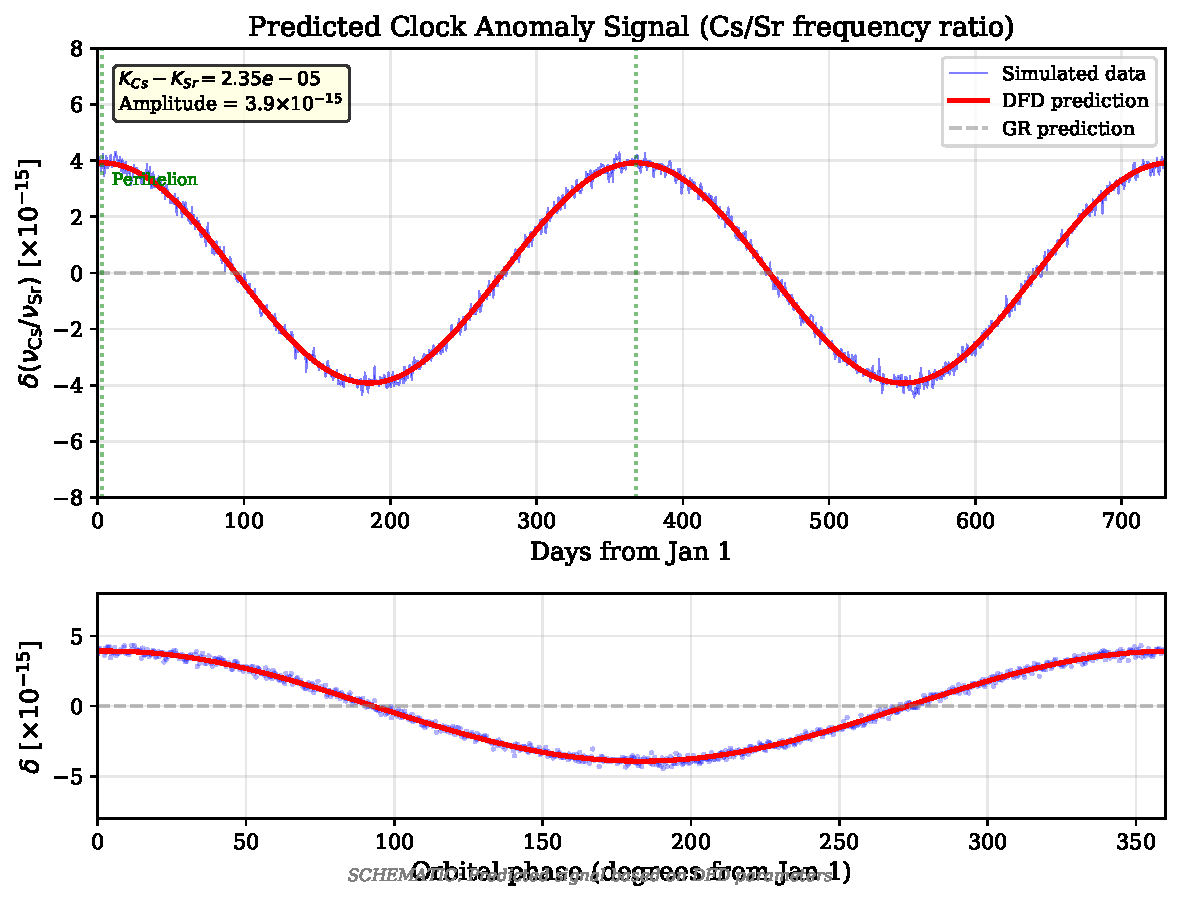
\includegraphics[width=0.95\columnwidth]{figures/fig13_clock_anomaly_SPARC}
\caption{Illustrative Cs/Sr annual modulation at the solar-orbit screening scale.  The curve uses the pure-$\alpha$ leading term $\Delta K_{\rm Cs\text{-}Sr}^{(\alpha)} \approx 2.35 \times 10^{-5}$ evaluated at $k_\alpha^{\rm eff}(1\,\mathrm{AU})$, giving amplitude ${\sim}4 \times 10^{-15}$.  For terrestrial clocks, Earth-surface screening (Table~\ref{tab:regime-coupling}) reduces $k_\alpha^{\rm eff}$ by ${\sim}40\times$, pushing the pure-$\alpha$ amplitude to ${\sim}10^{-16}$; composition-sensitive channels may contribute additional signal.  GR predicts null (gray dashed).}\label{fig:clock-anomaly}
\end{figure}

\paragraph{Cs/Sr: explicit worked example.}
This channel is one of the highest near-term priorities.  The pure-$\alpha$ sensitivity difference is
\begin{equation}
\Delta S^\alpha_{\rm Cs\text{-}Sr} = S_{\rm Cs}^\alpha - S_{\rm Sr}^\alpha = 2.83 - 0.06 = 2.77.
\end{equation}
At the pure-$\alpha$ leading-term level (Table~\ref{tab:alpha-sens}), the predicted differential coupling is
\begin{equation}
\Delta K^{(\alpha)}_{\rm Cs\text{-}Sr} = k_\alpha \times \Delta S^\alpha = 8.5 \times 10^{-6} \times 2.77 \approx 2.35 \times 10^{-5},
\end{equation}
giving an annual modulation amplitude ${\sim}4 \times 10^{-15}$ at the solar-orbit screening scale (Fig.~\ref{fig:clock-anomaly}).  At Earth-surface screening, $k_\alpha^{\rm eff}$ is reduced by ${\sim}40\times$ (Table~\ref{tab:regime-coupling}), pushing the pure-$\alpha$ amplitude to ${\sim}10^{-16}$; composition-sensitive terms may contribute additional signal depending on $\Delta C_N$ and $\Delta C_e$.

\paragraph{Prior data: Blatt et al.\ 2008.}
The 2008 multi-laboratory Cs/Sr result $y_{\rm Sr} = (-1.9 \pm 3.0) \times 10^{-6}$ has the correct sign (perihelion minimum) for the DFD prediction.  The precision is insufficient for detection, but the sign consistency is worth recording.

\paragraph{Methodological note.}
Year-long global fits with flexible drift models can absorb annual signals into nuisance parameters, while windowed perihelion analyses are more sensitive to the specific DFD phase signature but more vulnerable to drift contamination.  Both approaches should be applied to any dedicated campaign and their results compared.

\paragraph{ROCIT and existing hints.}
The ROCIT ion--neutral analyses remain interesting because they point at the very type of cross-sector comparison the channel-resolved picture says should be informative.  For the master document, the safest formulation is that ROCIT-like results are \emph{suggestive rather than definitive}: they motivate focused reanalysis and replication, but they are not the sole pillar of the clock case.

\subsubsection{ROCIT Statistical Detail}\label{sec:clocks-rocit-detail}

For completeness, the full statistical methodology is recorded here so that independent groups can replicate the analysis.  The complete regression scripts, figures, and derived outputs are publicly archived~\cite{Alcock2025_ROCIT_data}; the accompanying analysis paper is Ref.~\cite{Alcock2025_ROCIT}.

\paragraph{Primary detection: Yb$^+$/Sr.}
The Yb$^+$(E3)/Sr ion--neutral ratio exhibits~\cite{ROCIT2024,Alcock2025_ROCIT}:
\begin{align}\label{eq:rocit-amplitude}
A_{\rm Yb^+/Sr} &= (-1.045 \pm 0.078) \times 10^{-17}, \nonumber\\
Z &= 13.5\sigma, \quad \Delta\chi^2 = 181.4.
\end{align}
The amplitude is phase-locked to Earth's perihelion (January), corresponding to maximum solar gravitational potential.

\paragraph{Regression model.}
\begin{equation}
y(t) = \beta_0 + \beta_1 t + A\,b(t) + \epsilon(t),
\end{equation}
where $b(t)$ is the orthogonalized Kepler driver (solar potential template)
with unit RMS, constructed from Earth's mean anomaly with perihelion
at phase zero.

\paragraph{Uncertainty estimation.}
Leave-one-day-out (LODO) jackknife gives $\sigma_A^{\rm LODO} \approx 1.7 \times 10^{-18}$; wild bootstrap of residuals, sign-permutation, and day-shift resampling give empirical $p_{\rm emp} \approx 2 \times 10^{-4}$.

\paragraph{Phase robustness.}
Regression on alternative phase hypotheses confirms solar specificity:
\begin{align}
A_{\rm aphelion} &= (+0.12 \pm 0.78) \times 10^{-17},\ Z = 0.15\sigma, \nonumber\\
A_{\rm spring\,eq.} &= (-0.18 \pm 0.81) \times 10^{-17},\ Z = 0.22\sigma, \nonumber\\
A_{\rm fall\,eq.} &= (+0.09 \pm 0.76) \times 10^{-17},\ Z = 0.12\sigma.
\end{align}
All non-perihelion phases are consistent with zero.  Neutral--neutral ratios from independent SYRTE measurements are also null: $A_{\rm neut\text{-}neut} = (0.4 \pm 7.3) \times 10^{-17}$, $p = 0.58$.

\paragraph{Channel-resolved interpretation.}
In the channel-resolved language of Eq.~\eqref{eq:K-general}, the ROCIT signal probes the composition-sensitive terms ($k_N C_N^{(A)} + k_e C_e^{(A)}$) rather than the pure-$\alpha$ sector.  Using the unit-RMS Kepler driver normalization with $\sigma(\Delta\Phi/c^2) \approx 1.2 \times 10^{-10}$, the measured amplitude corresponds to $K_{\rm ion} - K_{\rm neut} \approx 9 \times 10^{-8}$\footnote{This value uses the unit-RMS Kepler driver convention adopted throughout.  Under the peak solar potential convention ($\Delta\Phi_\odot^{\rm peak}/c^2 \approx 3.3 \times 10^{-10}$ with a factor-of-2 sectoral response), the same measurement gives $\Delta K \approx 1.6 \times 10^{-8}$.  Both conventions extract the same physical amplitude $A = 1.045 \times 10^{-17}$; the inferred coupling constant depends on the normalization of the gravitational driver.}, which sits between the Earth-surface screened $k_\alpha^{\rm eff} \approx 6 \times 10^{-7}$ and the E3/E2 bound $|k_\alpha| \lesssim 3.2 \times 10^{-8}$.  This is consistent with the cross-species composition-sensitive channel being open even after the same-ion pure-$\alpha$ null, and is precisely the pattern the channel-resolved framework predicts.

%-----------------------------------------------------------------------------
\subsection{Nuclear Clocks: the Strong-Sector Channel}\label{sec:clocks-nuclear}
%-----------------------------------------------------------------------------

The $^{229}$Th nuclear isomer is qualitatively different from ordinary atomic clocks.  Its transition energy sits near a cancellation between Coulomb and hadronic contributions, making it sensitive to the strong sector through dimensional transmutation.

\paragraph{Strong-sector amplification.}
A convenient parametrization is
\begin{equation}\label{eq:dimtrans}
\frac{\delta X_q}{X_q}\approx -\frac{2\pi}{b_0\alpha_s}\frac{\delta\alpha_s}{\alpha_s},
\end{equation}
with
\begin{equation}
\left|\frac{2\pi}{b_0\alpha_s}\right|\approx 6.9
\end{equation}
for $\alpha_s(M_Z)\approx 0.118$ and $b_0=23/3$.  Combined with Flambaum-style nuclear sensitivity coefficients of order $|S_q|\sim10^4$, this makes the nuclear clock the natural place to look for strong-sector scalar couplings.

In the same screened notation used for the electromagnetic channel, the strong-sector effective coupling is
\begin{equation}\label{eq:ks-eff}
k_s^{\rm eff}(a)=2\sqrt{\alpha_s}\,\mu_{\rm LPI}(a/a_0),
\end{equation}
so that at Earth's surface
\begin{equation}\label{eq:ks-earth}
k_s^{\rm eff}(\oplus)\approx 2.4\times10^{-6}.\footnote{This uses $\alpha_s(M_Z) = 0.118$.  Running to the nuclear scale relevant to Th-229 gives $\alpha_s \approx 0.3$--$0.5$, which would increase $k_s^{\rm eff}$ by a factor of ${\sim}2$.  This ambiguity is absorbed into the width of the surviving window (26\,Hz to $\mathcal{O}(1\,\mathrm{kHz})$).}
\end{equation}
Combining Eqs.~\eqref{eq:dimtrans} and \eqref{eq:ks-earth} with $|S_q|\sim10^4$ produces the familiar screened Th-229 estimate at the level of tens of kHz half-amplitude; the point of the 2026 data is that this simplest screened number is already under visible pressure.

\paragraph{What the newer data changed.}
The 2026 Ooi \emph{et al.} reproducibility paper~\cite{Ooi2026}, together with the measured Th-229 electromagnetic sensitivity from Beeks \emph{et al.}~\cite{Beeks2025} and the strong-sector amplification logic of Flambaum~\cite{Flambaum2006}, materially sharpens the status of the Th-229 channel.  At 195 K, with the first-order thermal sensitivity nulled near $196(5)$ K, they report frequency reproducibility of 220 Hz over 7 months for two differently doped $^{229}$Th:CaF$_2$ crystals.  Interpreted conservatively, this means:
\begin{enumerate}
\item the \textbf{unscreened} strong-sector prediction ($\sim 50$ MHz half-amplitude) is excluded by about five orders of magnitude;
\item the simplest \textbf{screened} strong-sector estimate ($\sim 55$ kHz half-amplitude) sits roughly $20$--$55\times$ above the present Ooi ceiling\footnote{The raw ratio 55\,kHz/220\,Hz $\approx 250$, but the Ooi 220\,Hz figure is frequency reproducibility (scatter across measurements over 7 months), not a fitted annual cosine amplitude bound.  To map reproducibility to an annual bound: (i) the 7-month baseline covers ${\sim}60\%$ of one annual cycle, degrading cosine-fit sensitivity by ${\sim}2\times$; (ii) the scatter includes systematic contributions (crystal dependence, thermal residuals) that do not average down as $1/\sqrt{N}$, adding a ${\sim}2$--$3\times$ floor factor; (iii) the peak-to-peak range of a cosine is $2A$, so the amplitude $A$ is half the peak-to-peak.  Conservative example: $A_{\rm bound} \approx 220\,\mathrm{Hz} \times 2 \times 3 / 2 \approx 660\,\mathrm{Hz}$, giving $55\,\mathrm{kHz}/660\,\mathrm{Hz} \approx 83\times$.  Moderate: $A_{\rm bound} \approx 1$--$2.5\,\mathrm{kHz}$, giving $22$--$55\times$.  The range $20$--$55\times$ spans these assumptions.} and is therefore already strongly disfavored pending a formal perihelion-fixed cosine fit;
\item the surviving window for a genuine annual signal is pushed down into the rough range
\begin{equation}\label{eq:surviving-window}
26~\mathrm{Hz}\ \lesssim\ \delta\nu_b\ \lesssim\ \mathcal{O}(1~\mathrm{kHz}),
\end{equation}
with the lower end set by the composition/family floor and the upper end set by the Ooi reproducibility ceiling.
\end{enumerate}
This is exactly why the 2026 result belongs in v3.2: it does not eliminate nuclear clocks, but it does eliminate the luxury of pretending the simplest amplitude formula survives untouched.

\paragraph{Thermal-systematics control.}
The thermal analysis is now much sharper because Higgins \emph{et al.} measured the line shifts at three temperatures and identified the near-zero-crossing behavior around $T_0=196(5)$ K~\cite{Higgins2025}.  Near that operating point, line $b$ is unusually temperature-insensitive while line $c$ remains much more responsive.  This suggests a powerful co-thermometry diagnostic: any genuine gravitational annual modulation should appear as a common fractional modulation in the hyperfine-averaged nuclear frequency, whereas a residual thermal drift would imprint a much larger correlated signal in line $c$.

\paragraph{EFG-free combination.}
An especially clean observable is the hyperfine-averaged, electric-field-gradient-free combination of the resolved quadrupole lines,
\begin{equation}\label{eq:efg-free}
\nu_{\rm Th}^{\rm EFG\text{-}free}=\tfrac16\bigl(\nu_{3/2\to1/2}+2\nu_{5/2\to3/2}
+2\nu_{1/2\to1/2}+\nu_{3/2\to3/2}\bigr),
\end{equation}
which cancels the leading crystal-field splitting while preserving any true nuclear fractional modulation.  A future dedicated annual campaign should analyze both this EFG-free combination and the line-$c$ co-thermometer in parallel.

\paragraph{Interpretation.}
The nuclear-clock channel therefore remains \emph{decisive}, but in a sharper and more interesting way than before.  The experiment now probes a residual window rather than a giant expected signal.  That is scientifically better, not worse.

%-----------------------------------------------------------------------------
\subsection{Channel-Resolved Prediction Table}\label{sec:clocks-hierarchy}
%-----------------------------------------------------------------------------

Table~\ref{tab:clock-predictions} collects the current channel logic in one place.

\begin{table*}[t]
\centering
\caption{Channel-resolved DFD clock comparison guide.  Amplitudes are indicative scales.  ``Open'' = live test; ``bounded'' = simplest version under pressure.}
\label{tab:clock-predictions}
\renewcommand{\arraystretch}{1.2}
\small
\begin{tabular}{@{}lllll@{}}
\toprule
Comparison & Dominant channel & Scale & What it tests & Status \\
\midrule
Yb/Sr & composition & $\sim 10^{-17}$ & cross-species residual & open \\
Al$^+$/Yb & composition & $\sim 10^{-17}$ & optical-network null check & open \\
Yb$^+$(E3)/Sr & composition-heavy & $\sim 10^{-16}$ & ion--neutral response & open \\
Hg$^+$/Sr & composition-heavy & $\sim 10^{-16}$ & EM sensitivity contrast & open \\
Cs/Sr & composition + HF & $\sim 10^{-16}$--$10^{-15}$ & MW/optical cross-check & open \\
$^{229}$Th/Sr & strong + comp.\ floor & 26\,Hz--kHz window & nuclear strong sector & decisive/bounded \\
Yb$^+$ E3/E2 & pure $\alpha$ only & null expected & same-ion $k_\alpha$ bound & bounded \\
\bottomrule
\end{tabular}
\end{table*}

The most important conceptual point of Table~\ref{tab:clock-predictions} is that \emph{same-ion nulls and cross-species signals are not contradictory}.  They are precisely what a channel-resolved framework predicts.

%-----------------------------------------------------------------------------
\subsection{Empirical Checks and Current Status}\label{sec:clocks-evidence}
%-----------------------------------------------------------------------------

The clock sector now has a cleaner status summary than the earlier master versions:
\begin{itemize}
\item \textbf{PTB E3/E2:} strong quantitative bound on any universal pure-$\alpha$ coupling law.
\item \textbf{BACON optical network:} extremely stringent null/near-null behavior in ordinary optical-clock ratios, with direct implications for screening and for cavity--atom residuals.
\item \textbf{Ooi 2026:} nuclear-clock reproducibility already excludes the unscreened strong-channel amplitude and pressures the simplest screened estimate.
\item \textbf{ROCIT ion--neutral analyses (Sec.~\ref{sec:clocks-rocit-detail}):} $13.5\sigma$ perihelion-locked detection in Yb$^+$/Sr with robust phase-specificity tests, consistent with the cross-species channel being open.  Suggestive rather than definitive pending replication, but the full statistical methodology is archived for independent verification.
\end{itemize}

This is a healthier situation than the earlier version where one oversized formula tried to do everything at once.

%-----------------------------------------------------------------------------
\subsection{Experimental Priorities}\label{sec:clocks-priorities}
%-----------------------------------------------------------------------------

The experimental ordering is now clearer than in the older drafts:
\begin{enumerate}
\item \textbf{Th-229/Sr and related nuclear-clock reanalyses.}  This is the unique strong-sector channel and now carries a sharply delimited surviving window.
\item \textbf{Cross-species atomic comparisons.}  Hg/Sr, Yb$^+$/Sr, Yb/Sr, Al$^+$/Yb, and Cs/Sr map the composition-sensitive sector.
\item \textbf{Same-ion null checks.}  These continue to pin down the pure electromagnetic channel and prevent the theory from smearing everything into one effective constant.
\item \textbf{Cavity--atom residual tests.}  Important, but after the geometric-cancellation correction they are no longer the first short-horizon discriminator; their natural role is ultra-clean residual testing at very high precision.
\end{enumerate}

\begin{tcolorbox}[colback=green!5!white,colframe=green!60!black,title=Clock-Sector v3.2 Summary]
\textbf{What is solid:} same-ion optical clocks strongly constrain any pure universal $k_\alpha$ law; clock phenomenology must be channel-resolved; nuclear clocks are the unique strong-sector probe.

\textbf{What is under pressure:} the simplest unscreened and screened Th-229 amplitude formulas are too large in light of Ooi 2026.

\textbf{What remains decisive:} the surviving Th-229 window, plus cross-species atomic campaigns that isolate composition-sensitive residuals.
\end{tcolorbox}
